\subsection{Funções Limitadas}

\begin{definition}
    Seja $f: D \subset \R \to \R$ uma função.
\begin{enumerate}[(i)]
  \item $f$ é \textdef{limitada superiormente} se existe $M \in \R$ tal
  que $f(x) \leq M$ para todo $x \in D$;
  \item $f$ é \textdef{limitada inferiormente} se existe $M \in \R$ tal
  que $f(x) \geq M$ para todo $x \in D$;
  \item $x_0 \in D$ é um \textdef{ponto de máximo absoluto} de $f$ se
  $f(x_0) \geq f(x)$ para todo $x \in D$;
  \item $x_0 \in D$ é um \textdef{ponto de mínimo absoluto} de $f$ se
  $f(x_0) \leq f(x)$ para todo $x \in D$;
  \item $x_0 \in D$ é um \textdef{ponto de máximo local} de $f$ se
  existe $r>0$ tal que $f(x_0) \geq f(x)$ para todo $x \in D \cap \paren{x_0 - r , x_0+r}$;
  \item $x_0 \in D$ é um \textdef{ponto de mínimo local} de $f$ se
  existe $r>0$ tal que $f(x_0) \leq f(x)$ para todo $x \in D \cap \paren{x_0 - r ,
  x_0+r}$.
\end{enumerate}
\end{definition}

\begin{example}
    A função $h : \left( -1 ; 6 \right] \to \R$, cujo gráfico é esboçado
na Imagem~\ref{img:funcao-h-descontinua}, é definida por:
%
$$h(x) = \begin{cases}
                                3x-x^2 & \ \text{ se } \ x\leq 2 \\
                                \modu{x-4} +1 & \ \text{ se } \ 2 < x \leq 5 \\
                                2 & \ \text{ se } \ x > 5 \\
                                \end{cases}.$$
%
\begin{figure}
\centering
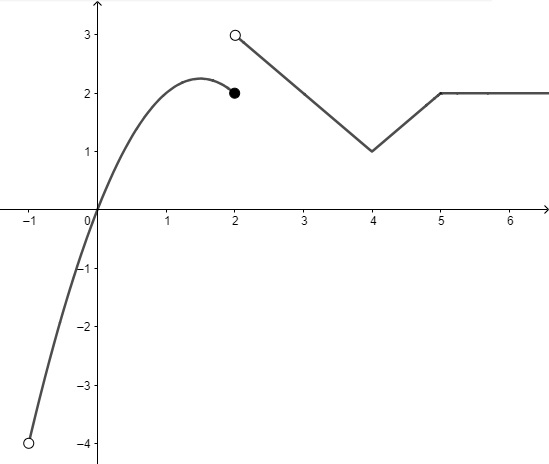
\includegraphics[scale=0.5]{\imgdirfromsection/funcao-h-descontinua}
\caption{Gráfico da função $h$.}
\label{img:funcao-h-descontinua}
\end{figure}
%
Identifique, pelo gráfico, os intervalos de monotonicidade e os extremos locais e absolutos $h$.
\end{example}

\begin{solution}
    A partir do gráfico, pode-se perceber que a função $h$ é crescente nos intervalos $(-1;1{,}5]$ e $[4;5]$,
    decrescente em $[1,5; 2]$ e $(2;4]$ e constante em $[5;+\infty]$. 
    Note que o número 4 está presente tanto em um intervalo de crescimento quanto em um de decrescimento,
    e o 5 está num dos intervalos de decrescimento e no de constância da função.
    
    Também por observação do gráfico da função, conclui-se que o ponto $(1{,}5; 2{,}25)$ é um mínimo local, e o ponto $(4,1)$ é um máximo local.
    A função não possui máximos ou mínimos locais.
\end{solution}

\begin{onlineact}
    \khan{https://pt.khanacademy.org/math/algebra/algebra-functions/positive-negative-increasing-decreasing-intervals/e/increasing-decreasing-intervals-of-functions}
    {Intervalos Crescentes e Decrescentes}.
\end{onlineact}

\begin{onlineact}
    \khan{https://pt.khanacademy.org/math/algebra/algebra-functions/maximum-and-minimum-points/e/recognize-maxima-and-minima}
    {Mínimos e Máximos Relativos}.
\end{onlineact}

\begin{onlineact}
    \khan{https://pt.khanacademy.org/math/algebra/algebra-functions/maximum-and-minimum-points/e/recognize-absolute-maxima-and-minima}
    {Mínimos e Máximos Absolutos}.
\end{onlineact}